\documentclass[a4paper]{article}
\usepackage[utf8]{inputenc}


%=-=-=-=-=-=-=-=-=-=-=-=-=-=-=-=-=-=-=-=-=-=-=-=-=-=-=-=-=-=-=-=-=-=-=-=-=-=-=-=-
% PREAMBLE
%=-=-=-=-=-=-=-=-=-=-=-=-=-=-=-=-=-=-=-=-=-=-=-=-=-=-=-=-=-=-=-=-=-=-=-=-=-=-=-=-

%%%%%%%%%%%%%%%%%%%%%%%%%%%%%%%%%%%%%%%%%%%%%%%%%%%%%%%%%%%%%%%%%%%%%
% Important styling notes
%%
% For now, to include img.jpg in img/path/to/img.jpg, just use:
% path/to/img.jpg - for details see style.tex
%=-=-=-=-=-=-=-=-=-=-=-=-=-=-=-=-=-=-=-=-=-=-=-=-=-=-=-=-=-=-=-=-=-=-=-=-=-=-=-=-
% Packages
%%
%\usepackage{fullpage} % Package to use full page
\usepackage[top=1in,bottom=1in,left=1in,right=0.7in,heightrounded]{geometry}

\usepackage{parskip}                    % Package to tweak paragraph skipping
\usepackage{amsmath}                    % standard
\usepackage{amssymb}                    % standard - Double R symbol etc.
\usepackage{hyperref}
\usepackage{amsthm}                     % standard - theorem, definition, etc.
\usepackage{multicol}                   % multiple columns for numbering
\usepackage{enumitem}                   % standard - enumerate styles
\usepackage[utf8]{inputenc}
\usepackage{scrextend}                  % indentation
\usepackage{graphicx}                   % standard - add figures
\usepackage{float}                      % standard - figure position, use [H] option
\usepackage{pifont}                     % symbols
\usepackage{gensymb}                    % degree symbol \degree
\usepackage{xcolor}                     % bg color
\hypersetup{
    colorlinks,
    linkcolor={black!50!black},
    citecolor={blue!50!black},
    urlcolor={blue!80!black}
}
\usepackage{framed}                     % bg color
\usepackage[T1]{fontenc}                % small caps
\usepackage{sectsty}                    % headings colour
\usepackage{mathtools}                  % Loads amsmath
\usepackage{amsthm,thmtools,xcolor}     % coloured theorem
\usepackage[toc,page]{appendix}         % reference to appendix
%\usepackage{titlesec}                   % change chapter, section, etc. formats
\usepackage{xifthen}                    % if, else
\usepackage{etoolbox}
% format numbering in theorem, lemma, etc. environment
\AtBeginEnvironment{theorem}{\setlist[enumerate, 1]{font=\upshape,  wide=0.5em, before=\leavevmode}}
\AtBeginEnvironment{lemma}{\setlist[enumerate, 1]{font=\upshape,  wide=0.5em, before=\leavevmode}}
\usepackage[letterspace=150]{microtype} % \textls{<letterspaced text>} % 0 <= letterspace <= 1000, 1000 = M space
\usepackage{letltxmacro}                % renew commands?
\usepackage{minted}                     % package to list code
    % otherwise minted goes off the page
    \setmintedinline{breaklines}
\usepackage{subfig}
\usepackage{eso-pic}                    % title page bg pic
\usepackage{varwidth}
\PassOptionsToPackage{svgnames}{xcolor}
\usepackage{fontawesome}                % \faQuestionCircle
\usepackage{marvosym}                   %\Pointinghand
\usepackage{mdframed}                   % easy outline frames
\usepackage[many]{tcolorbox}            % colour box for theorem styles
\usepackage{array,booktabs,calc} % table figs and text
\usepackage{comment}                    % \begin{comment}
\usepackage{fancyhdr}                   % page headings
\usepackage{mdframed}                   % boxes
\usepackage[backend=biber,sorting=none,style=ieee]{biblatex}
\usepackage{caption}
%%% caption options {
%\DeclareCaptionFont{white}{\color{white}}
\DeclareCaptionFormat{listing}{\colorbox{magenta!30!gray}{\parbox{\textwidth}{#1#2#3}}}
\captionsetup[lstlisting]{format=listing,labelfont={bf,small},textfont=small,skip=-1pt}
%%% }
\addbibresource{bibliography.bib}
\usepackage{url}
\usepackage{textcomp}
\usepackage[makeroom]{cancel}            % crossed symbols
\usepackage{algorithm}
\usepackage[noend]{algpseudocode}
\usepackage{tikz}
\usetikzlibrary{arrows.meta,positioning,quotes} % arrows and nodes in tikz
\usepackage{marginnote}
\usepackage{pgfplots}
\usepackage{pstricks-add,pst-slpe}  % for fancy tikz arrows
%\usepackage{titlesec}                   % title style
\usepackage{lmodern}                    % a font
\usepackage{titletoc} % Required for manipulating the table of contents
\usepackage{titlesec} % Allows customization of titles
\usepackage{fouriernc} % Use the New Century Schoolbook font
\usepackage{booktabs} % things in page margins
\usepackage{stmaryrd } % \varoast
\usepackage{listings} % code listings
\usepackage{longtable} % table across multiple pages
\usepackage{styles/nasm/lang}  % include custom language for NASM assembly.
\usepackage{styles/nasm/style} % include custom style for NASM assembly.



%% extra comments that I don't know where they belong:
% list of ding tags: http://willbenton.com/wb-images/pifont.pdf

%=-=-=-=-=-=-=-=-=-=-=-=-=-=-=-=-=-=-=-=-=-=-=-=-=-=-=-=-=-=-=-=-=-=-=-=-=-=-=-=-
% Colours for various things
%%


\definecolor{shadecolor}{rgb}{1.,0.933,0.96} % bg color, r,g,b <= 1
\definecolor{medium_blue}{RGB}{60,125,190}
\definecolor{dark_blue}{RGB}{25,60,85}
\definecolor{dark_red}{RGB}{77,16,16}
\definecolor{LightPink}{rgb}{0.92.,0.8,0.84} % bg color, r,g,b <= 1
\definecolor{LighterPink}{rgb}{1.,0.94,0.97} % bg color, r,g,b <= 1
\definecolor{LightestPink}{rgb}{1.,0.95,0.99} % bg color, r,g,b <= 1
\definecolor{DarkestPink}{rgb}{0.36, 0.0, 0.18}
\definecolor{DarkerPink}{rgb}{0.41, 0.0, 0.21}
\definecolor{DarkPink}{rgb}{0.55, 0.05, 0.37}
\definecolor{lightestestpink}{RGB}{255,248,252}
\definecolor{codegray}{rgb}{0.5,0.5,0.5}
\definecolor{codegrayblue}{rgb}{0.35,0.35,0.47}



%=-=-=-=-=-=-=-=-=-=-=-=-=-=-=-=-=-=-=-=-=-=-=-=-=-=-=-=-=-=-=-=-=-=-=-=-=-=-=-=-
% Define my own theorem styles
%%

% "base" styles
\declaretheoremstyle[
  headfont=\color{DarkPink}\bfseries,
  bodyfont=\itshape,
]{colored}

\declaretheoremstyle[
  headfont=\color{DarkPink}\bfseries,
  bodyfont=\normalfont,
]{colored_upright}

% theorems (corollaries, etc) themselves, inherit from my style above
% Usage:
% \begin{theorem} \end{theorem}, \begin{lemma} \end{lemma}, ...
\declaretheorem[
	numberwithin=section,
 	style=colored,
	name=\textsc{Theorem},
]{theorem}

\tcolorboxenvironment{theorem}{
  boxrule=0pt,
  boxsep=2pt,
  colback={magenta!25!white},
  colframe=DarkPink,
  enhanced jigsaw, 
  borderline west={2pt}{0pt}{DarkPink},
  sharp corners,
  before skip=5pt,
  after skip=5pt,
  breakable,
  right=0mm % for equations
}

\declaretheorem[
	numberwithin=section,
 	style=colored,
	name=\textsc{Corollary},
]{corollary}

\tcolorboxenvironment{corollary}{
  boxrule=0pt,
  boxsep=1pt,
  colback={magenta!10!white},
  colframe=DarkPink,
  enhanced jigsaw, 
  borderline west={2pt}{0pt}{DarkPink},
  sharp corners,
  before skip=5pt,
  after skip=5pt,
  breakable,
  right=0mm % for equations
}

\declaretheorem[
	numberwithin=section,
	style=colored,
	name=\textsc{Lemma},
]{lemma}

\tcolorboxenvironment{lemma}{
  boxrule=0pt,
  boxsep=1pt,
  colback={magenta!10!white},
  colframe=DarkPink,
  enhanced jigsaw, 
  borderline west={2pt}{0pt}{DarkPink},
  sharp corners,
  before skip=5pt,
  after skip=5pt,
  breakable,
  right=0mm % for equations
}

\declaretheorem[
	numberwithin=section,
	style=colored,
	name=\textsc{Definition},
]{definition}

\tcolorboxenvironment{definition}{
  boxrule=0pt,
  boxsep=1pt,
  colback={magenta!25!white},
  colframe=DarkPink,
  enhanced jigsaw, 
  borderline west={2pt}{0pt}{DarkPink},
  sharp corners,
  before skip=5pt,
  after skip=5pt,
  breakable,
  right=0mm % for equations
}

\declaretheorem[
	numberwithin=section,
  	style=colored,
  	name=\textsc{Example},
]{exmp}

\declaretheorem[
	numberwithin=section,
  	style=colored,
  	name=\textsc{Solution},
]{soln}

%%% code listings
\lstdefinestyle{code1}{
    backgroundcolor=\color{lightestestpink},   
    commentstyle=\color{codegrayblue},
    keywordstyle=\color{DarkerPink},
    numberstyle=\tiny\color{codegray},
    stringstyle=\color{black!40!cyan},
    basicstyle=\small\ttfamily,
    breakatwhitespace=false,
    breaklines=true,        
    captionpos=t,             
    keepspaces=true,        
    numbers=left,           
    numbersep=5pt,
    showspaces=false, 
    showstringspaces=false,
    showtabs=false,
    tabsize=4
}

\lstset{style=code1}

%=-=-=-=-=-=-=-=-=-=-=-=-=-=-=-=-=-=-=-=-=-=-=-=-=-=-=-=-=-=-=-=-=-=-=-=-=-=-=-=-
% Headers (size, font, colour)
%%




\makeatletter
\renewcommand{\@seccntformat}[1]{\llap{\textcolor{DarkestPink}{\csname the#1\endcsname}\hspace{1em}}}                    
\renewcommand{\section}{\@startsection{section}{1}{\z@}
{-4ex \@plus -1ex \@minus -.4ex}
{1ex \@plus.2ex }
{\normalfont\large\sffamily\bfseries\textcolor{DarkestPink}}}
\renewcommand{\subsection}{\@startsection {subsection}{2}{\z@}
{-3ex \@plus -0.1ex \@minus -.4ex}
{0.5ex \@plus.2ex }
{\normalfont\sffamily\bfseries\textcolor{DarkestPink}}}
\renewcommand{\subsubsection}{\@startsection {subsubsection}{3}{\z@}
{-2ex \@plus -0.1ex \@minus -.2ex}
{.2ex \@plus.2ex }
{\normalfont\small\sffamily\bfseries\textcolor{DarkestPink}}}                        


%=-=-=-=-=-=-=-=-=-=-=-=-=-=-=-=-=-=-=-=-=-=-=-=-=-=-=-=-=-=-=-=-=-=-=-=-=-=-=-=-
% Numberings, counters and spacings
%%
\numberwithin{equation}{section} % section number in eq/s
\setlength{\jot}{7pt} % spacing in split, gathered env/s



%% Custom examples
%% Output - Example 1,2,...
\newcounter{example}
\newenvironment{example}[1][]{\refstepcounter{example}\par\medskip
   \textbf{Example~\theexample. #1} \rmfamily}{\medskip}
%%%%%%%%%%%% End of unused %%%%%%%%%%%%



%=-=-=-=-=-=-=-=-=-=-=-=-=-=-=-=-=-=-=-=-=-=-=-=-=-=-=-=-=-=-=-=-=-=-=-=-=-=-=-=-
% Paths
%%
\graphicspath{ {./img/} } % figures' path - can look up files directly from there


%=-=-=-=-=-=-=-=-=-=-=-=-=-=-=-=-=-=-=-=-=-=-=-=-=-=-=-=-=-=-=-=-=-=-=-=-=-=-=-=-
% User defined macros (math mode)
%%


% Curly braces under text. Usage: \myunderbrace{upper}{lower}
\newcommand{\myunderbrace}[2]{\mathrlap{\underbrace{\phantom{#1}}_{#2}} #1}
\newcommand{\setR}{\mathbb{R}} % \ouble R
\newcommand{\setRn}{\mathbb{R}^n} %  double R^n
\newcommand{\setN}{\mathbb{N}} % double N
\newcommand{\setZ}{\mathbb{Z}} % double Z
\let\oldemptyset\emptyset
\let\emptyset\varnothing % nice - looking empty set symbol
\newcommand{\fancyN}{\mathcal{N}} % null space
\newcommand{\fancyR}{\mathcal{R}} % range

\newcommand{\bx}{\textbf{x}}
\newcommand{\by}{\textbf{y}}
\newcommand{\bb}{\textbf{b}}
\newcommand{\bA}{\textbf{A}}
\newcommand{\bB}{\textbf{B}}
\newcommand{\bI}{\textbf{I}}
% double bars as in norm
\newcommand{\norm}[1] {\lVert #1 \rVert} 
\newcommand{\trans}[1]{#1^{\top}}

\newcommand{\mean}[1]{\bar{#1}}
\newcommand{\var}{\sigma^2}

\newcommand{\partdevx}[1]{\frac{\partial #1}{\partial x}}
\newcommand{\partdevxx}[1]{\frac{\partial #1}{\partial x}}
\newcommand{\partdevxn}[1]{\frac{\partial^n #1}{\partial x^n}}
\newcommand{\partdevy}[1]{\frac{\partial #1}{\partial x}}
\newcommand{\partdevyy}[1]{\frac{\partial #1}{\partial y}}
\newcommand{\partdevyn}[1]{\frac{\partial^n #1}{\partial y^n}}

% text above = symbol
\newcommand{\overeq}[1]{\ensuremath{\stackrel{#1}=}} 
\newcommand{\greatersmaller}{%
  \mathrel{\ooalign{\raisebox{.6ex}{$>$}\cr\raisebox{-.6ex}{$<$}}}
} % greater and smaller symbols on top of each other, same line

%=-=-=-=-=-=-=-=-=-=-=-=-=-=-=-=-=-=-=-=-=-=-=-=-=-=-=-=-=-=-=-=-=-=-=-=-=-=-=-=-
% User defined macros (non math)

\newcommand{\qedblack}{$\hfill\blacksquare$} % black square end of line
\newcommand{\qedwhite}{\hfill \ensuremath{\Box}} % white square end of line
\newcommand{\hquad}{\hskip0.5em\relax}% half quad space
%\newcommand{\TODO}{\textcolor{red}{\bf TODO!}\;}

\newcommand{\TODO}[1][]{%
    \ifthenelse{\equal{#1}{}}{\textcolor{red}{\bf TODO!}\;}{\textcolor{red}{\textbf {TODO:} #1}\; }%
}
\newcommand{\B}[1]{\textbf{\textup{#1}}} % bold and upright
\renewcommand{\labelitemi}{\scriptsize$\textcolor{DarkPink}{\blacksquare}$} % itemize - squares instead of bullets
\newcommand{\emphasis}[1]{\textls{#1}}

\LetLtxMacro{\originaleqref}{\eqref}
\renewcommand{\eqref}{Eq.~\originaleqref}
\renewcommand*{\eqref}[1]{Eq.~\originaleqref{#1}}





% background images
%%%%%%%
\newcommand\BackgroundPic{%
\put(0,0){%
\parbox[b][\paperheight]{\paperwidth}{%
\vfill
%\centering

\includegraphics[width=0.125\paperwidth,height=\paperheight,%
]{img/background_02.png}% use ,keepaspectratio
\vfill
}}}
%%%%%%%
% end of background image
%%%%%%%%%%%%%% my own frame
\newmdenv[topline=false,bottomline=false]{leftrightbox}
%%%%%%%%%%%%% end
%%%%%%%%%%%%% my own comment
\newcommand{\mycomment}[1]{\begin{leftrightbox}\Pointinghand~\textbf{Comment:}~#1 \end{leftrightbox}}
%%%%%%%%%%%%% end
% my custom note https://tex.stackexchange.com/questions/301993/create-custom-note-environment-with-tcolorbox
\newmdenv[
    topline=false,
    bottomline=false,
    rightline=false,
    innerrightmargin=0pt
]{siderule}
\newenvironment{mynote}%
    {\begin{siderule}\textbf{\Pointinghand~Note:}}
    {\end{siderule}}
%%%%%%%%%%%%% my own box
\newcommand{\boxone}[1]{\begin{tcolorbox}[colback = LighterPink,colframe=LightPink]
#1
\end{tcolorbox}}
%%%%%%%%%%%%% end

\let\oldemptyset\emptyset
\let\emptyset\varnothing
%algorithmic
\algdef{SE}[DOWHILE]{Do}{doWhile}{\algorithmicdo}[1]{\algorithmicwhile\ #1}%






\begin{document}
%=-=-=-=-=-=-=-=-=-=-=-=-=-=-=-=-=-=-=-=-=-=-=-=-=-=-=-=-=-=-=-=-=-=-=-=-=-=-=-=-
% GLOBAL STYLES (DOCUMENT SCOPE)
%=-=-=-=-=-=-=-=-=-=-=-=-=-=-=-=-=-=-=-=-=-=-=-=-=-=-=-=-=-=-=-=-=-=-=-=-=-=-=-=-
% caption: Figure 1 -> <bold> Fig. 1 </bold>
\captionsetup[figure]{labelfont={bf},labelformat={default},labelsep=period,name={Fig.}}


%=-=-=-=-=-=-=-=-=-=-=-=-=-=-=-=-=-=-=-=-=-=-=-=-=-=-=-=-=-=-=-=-=-=-=-=-=-=-=-=-
% TITLE PAGE
%=-=-=-=-=-=-=-=-=-=-=-=-=-=-=-=-=-=-=-=-=-=-=-=-=-=-=-=-=-=-=-=-=-=-=-=-=-=-=-=-
%%%%%%%%%%%%%%%%%%%%%%%%%%%%%%%%%%%%%%%%%
% Formal Book Title Page
% LaTeX Template
% Version 2.0 (23/7/17)
%
% This template was downloaded from:
% http://www.LaTeXTemplates.com
%
% Original author:
% Peter Wilson (herries.press@earthlink.net) with modifications by:
% Vel (vel@latextemplates.com)
%
% License:
% CC BY-NC-SA 3.0 (http://creativecommons.org/licenses/by-nc-sa/3.0/)
% 
% This template can be used in one of two ways:
%
% 1) Content can be added at the end of this file just before the \end{document}
% to use this title page as the starting point for your document.
%
% 2) Alternatively, if you already have a document which you wish to add this
% title page to, copy everything between the \begin{document} and
% \end{document} and paste it where you would like the title page in your
% document. You will then need to insert the packages and document 
% configurations into your document carefully making sure you are not loading
% the same package twice and that there are no clashes.
%
%%%%%%%%%%%%%%%%%%%%%%%%%%%%%%%%%%%%%%%%%

%----------------------------------------------------------------------------------------
%	PACKAGES AND OTHER DOCUMENT CONFIGURATIONS
%----------------------------------------------------------------------------------------



%----------------------------------------------------------------------------------------
%	TITLE PAGE
%----------------------------------------------------------------------------------------



\begin{titlepage} % Suppresses headers and footers on the title page

	\centering % Centre everything on the title page
	
	\scshape % Use small caps for all text on the title page
	
	\vspace*{\baselineskip} % White space at the top of the page
	
	%------------------------------------------------
	%	Title
	%------------------------------------------------
	
	\rule{\textwidth}{1.6pt}\vspace*{-\baselineskip}\vspace*{2pt} % Thick horizontal rule
	\rule{\textwidth}{0.4pt} % Thin horizontal rule
	
	\vspace{0.75\baselineskip} % Whitespace above the title
	
	{\LARGE COMPUTER VISION NOTES\\ \Large OBJECT LOCALISATION AND TRACKING\\} % Title
	
	\vspace{0.75\baselineskip} % Whitespace below the title
	
	\rule{\textwidth}{0.4pt}\vspace*{-\baselineskip}\vspace{3.2pt} % Thin horizontal rule
	\rule{\textwidth}{1.6pt} % Thick horizontal rule
	
	\vspace{2\baselineskip} % Whitespace after the title block
	
	%------------------------------------------------
	%	Subtitle
	%------------------------------------------------
	My personal notes on
	
	\vspace*{3\baselineskip} % Whitespace under the subtitle
	
	Object Localisation Techniques; Colour Matching, Mean Shift Tracking, Optical Flow, Lukas Kanade 
	
	\vspace*{3\baselineskip} % Whitespace under the subtitle
	
	%------------------------------------------------
	%	Editor(s)
	%------------------------------------------------
	
	By
	
	\vspace{0.5\baselineskip} % Whitespace before the editors
	
	{\normalfont \Large \mintinline{latex}{0xLeo} (\url{github.com/0xleo}) \\} % Editor list
	
	\vspace{0.5\baselineskip} % Whitespace below the editor list
	
	%\textit{The University of California \\ Berkeley} % Editor affiliation
	
	\vfill % Whitespace between editor names and publisher logo
	
	%------------------------------------------------
	%	Publisher
	%------------------------------------------------
	
	
	\vspace{0.3\baselineskip} % Whitespace under the publisher logo
	
	\today % Date
	
	{DRAFT X.YY} % Draft version
	{\\Missing: \ldots}

\end{titlepage}

%----------------------------------------------------------------------------------------

%\maketitle



%=-=-=-=-=-=-=-=-=-=-=-=-=-=-=-=-=-=-=-=-=-=-=-=-=-=-=-=-=-=-=-=-=-=-=-=-=-=-=-=-
% MAIN DOCUMENT
%=-=-=-=-=-=-=-=-=-=-=-=-=-=-=-=-=-=-=-=-=-=-=-=-=-=-=-=-=-=-=-=-=-=-=-=-=-=-=-=-
\newpage
\tableofcontents
\newpage



%------------------------------ New section ------------------------------%
\section{Writing a tiny bootloader}


\subsection{The power up}

As soon as the magical power button is pressed on the computer, it starts working. The motherboard sends a signal to the power supply device. After receiving the signal, the power supply provides the proper amount of electricity to the computer. Once the motherboard receives the power good signal, it tries to start the CPU. The CPU resets all leftover data in its registers and sets up predefined values for each of them \cite{linuxinsides}.

The 80386 CPU and later CPUs define the following predefined data in CPU registers after the computer resets:
\begin{verbatim}
IP          0xfff0
CS selector 0xf000
CS base     0xffff0000
\end{verbatim}

\subsection{Reset vector}
The job of these register values is to form the next instruction on the address but, which in this case is called \emphasis{reset vector}. Reset vector is part (one of the two) of the BIOS ROM. In turn, the reset vector contains some simple code which jumps to the main BIOS, where the CPU enters in \emphasis{real mode}. 

\subsection{Real mode -- entering the BIOS}
In real mode (App. \TODO), the registers can only address 1 MB ($2^{20} bytes$)of memory. Becuase the 8086 registers are 16-bit, each can address only $2^{16}$ bytes (64 kB). One register cannot achieve that, therefore two are used, and the method to obtain the physical address is called \emphasis{memory segmentation} (App. \TODO). Memory segmentation is used to make use of all the address space available. All memory is divided into small, fixed-size segments of 65536 bytes (64 KB). Since we cannot address memory above 64 KB with 16-bit registers, an alternate method was devised. The physical address is obtained given a segment selector register (REG) and an offset register (OFF) as:
\begin{equation}
	PHY=16\cdot SEG + OFF
\end{equation}

To prevent addressing locations higher than $2^{20}$ bytes, only the first 20 bits of the data address bus are used, called lines A0-A19. Line A20 therfore has special importance and is disabled in real mode (App. \TODO). Now the BIOS starts, as mentioned before in real mode.

\subsection{BIOS structure and flow}
After initializing and checking the hardware, the BIOS needs to find a bootable device. A boot order is stored in the BIOS configuration, controlling which devices the BIOS attempts to boot from. When attempting to boot from a hard drive, the BIOS tries to find a boot sector. On hard drives partitioned with an \emphasis{MBR partition layout} (App. \TODO), the boot sector is stored in the first 446 bytes of the first sector, where each sector is 512 bytes. The final two bytes of the first sector are 0x55 and 0xaa (signature bytes), which designates to the BIOS that this device is bootable. If these bytes are read, then the BIOS will jump to address 0x7c00, transferring control to the bootloader.

\subsection{Writing a bootloader}
We will write the first part of the BIOS following the instructions from Alex Parker's tutorial \cite{parkertut}.  
% ref http://3zanders.co.uk/2017/10/13/writing-a-bootloader/
Let’s get hello world printing to the screen. To do this we’re going to use the ‘Write Character in TTY mode’ BIOS Interrupt Call and the load string byte instruction lobsb which loads byte at address ds:si into al. Here goes:

\lstinputlisting[language=nasm,style=nasm,caption={Hello world bootloader. (\detokenize{src/boot.nasm)}.}, label=src:bot]{src/boot.nasm}

This is compiled by nasm (Nasm assembler details in the code explained in App \TODO) by:
\begin{verbatin}
$ nasm -f bin boot.nasm -o boot.bin
\end{verbatin}
The executable code is padded with zeros and ends with the signature bytes as desired, which is seen by running 
\begin{verbatim}
$ hexdump boot.bin
0000000 10be b47c ac0e c008 0474 10cd f7eb f4fa
0000010 6548 6c6c 206f 6f77 6c72 2164 0000 0000
0000020 0000 0000 0000 0000 0000 0000 0000 0000
*
00001f0 0000 0000 0000 0000 0000 0000 0000 aa55
\end{verbatim}
The last step is to run this bootloader by telling qemu to boot from a floppy disk:
\begin{verbatim}
$ qemu-system-x86_64 -fda boot1.bin	
\end{verbatim}
The result is:
\begin{figure}[H]
	\centering
	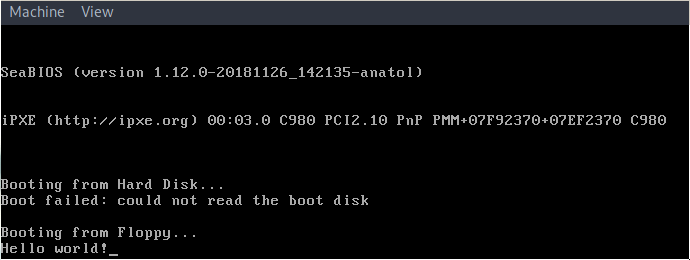
\includegraphics[width=0.8\linewidth]{qemu_boot.png}
	\caption{Booting the executable with qemu.}
\end{figure}

%=-=-=-=-=-=-=-=-=-=-=-=-=-=-=-=-=-=-=-=-=-=-=-=-=-=-=-=-=-=-=-=-=-=-=-=-=-=-=-=-
% Appendices
%=-=-=-=-=-=-=-=-=-=-=-=-=-=-=-=-=-=-=-=-=-=-=-=-=-=-=-=-=-=-=-=-=-=-=-=-=-=-=-=-
\newpage
\appendix

\section{Appendices}

% ------------------------ New appendix ------------------------ %
\newpage
\subsection{The need of memory segmentation in 8086}
%\label{app:my_cool_appendix}

\subsubsection{Virtual to physical address}
% ref http://www.ques10.com/p/32752/what-are-the-advantages-of-memory-segmentation-of-/
Segmentation means dividing the memory into logically different parts called segments. 8086 has a 20-bit address bus, often referred to as A0-19, hence it can access $2^{20}=1 MB$ memory, i.e.\ addresses from 0 to $2^{20}-1 = FFFFF \;\; H$. Intel's 8086 model uses 16-bit registers and using one such register it can access up to $2^{16}$ memory locations. Two registers 16-bit registers are used to address the whole physical memory, called \emphasis{segment register} (SEG) and \emphasis{offset register} (OFF). The 1 MB of physical memory must be divided in 16 logical blocks of 64 kB each. So to get the physical address, we multiply SEG by 16 and add OFF to get the exact offset;

% ref https://books.google.gr/books?id=pDGnxFyejN4C&pg=PA170&lpg=PA170&dq=8086+how+does+segmentation+16+bit+address+20+bit+work&source=bl&ots=DBZhIdco_5&sig=ACfU3U3NzHceWMlFCnISDCXdlS4wcEiktw&hl=en&sa=X&ved=2ahUKEwjbkvnQq-nhAhUcwsQBHfHqDD44ChDoATAIegQICRAB#v=onepage&q=8086%20how%20does%20segmentation%2016%20bit%20address%2020%20bit%20work&f=true
\begin{equation}
	PHY = 16*SEG + OFF = 10\ H * SEG + OFF 
\end{equation}

Note that in the hardware, multiplication of SEG by 16 is implemented by left shift by 4 so the previous equation can be rewritten:

\begin{equation}
	PHY = SEG << 4 + OFF
\end{equation}

The physical memory is divided into 4 segments, each which has a fixed base address (starting address) and a role;

\begin{itemize}
	\item Code Segment (CS)
\item Stack Segment (SS)
 \item Data Segment (DS)
 \item Extra Segment (ES)
\end{itemize}
% ref https://www.quora.com/How-is-a-20-bit-physical-memory-address-calculated-in-the-8086-microprocessor
\begin{exmp}
	Suppose the Data Segment holds the Base Aaddress as 1000 H and the data you need is present in the 0020 H memory location (Offset) of the Data Segment
\end{exmp}
\begin{soln}
Base address is multiplied by 16. Write it in binary and left shift it by 4 to find the product.
	\begin{minted}{python}
		SEG = 1000 H
		1000 H 	= 0001 0000 0000 b
		1000 H * 16 =
				= 0001 0000 0000 b << 4
				= 0001 0000 0000 0000 b
	\end{minted}
	Now add to it the offset \mintinline{python}{20 H = 10 0000 b}
	\begin{minted}{python}
				0001 0000 0000 0000 b
		 	+	0000 0000 0010 0000 b
			  = 0001 0000 0010 0000 b
			  = 10020 H
	\end{minted}
	That's the final physical address.
	\qedblack
\end{soln}
% ref https://books.google.gr/books?id=pDGnxFyejN4C&pg=PA170&lpg=PA170&dq=8086+how+does+segmentation+16+bit+address+20+bit+work&source=bl&ots=DBZhIdco_5&sig=ACfU3U3NzHceWMlFCnISDCXdlS4wcEiktw&hl=en&sa=X&ved=2ahUKEwjbkvnQq-nhAhUcwsQBHfHqDD44ChDoATAIegQICRAB#v=onepage&q=8086%20how%20does%20segmentation%2016%20bit%20address%2020%20bit%20work&f=true

Finally, a single physical address can be represented by many different segment and offset address combinations. For instance, for the virtual address \mintinline{latex}{0040:0049}, the physical address is \mintinline{latex}{40H * 16 + 49H = 449 H} (when we multiply by 16 in decimal -- 10 in hex, we simply add a 0 at the end, similar to multiplying with 10 in decimal). The same address can be represted by the segment:offset pair \mintinline{latex}{0000:0449H}.

Segmented memory is a nice way to give 8086 programs more memory than they would normally be able to access using 16-bit registers.
%\lstinputlisting[language=python,caption={A code listing (\detokenize{src/foo_bar.py)}.}, label=src:mylabel]{src/foo_bar.py}

\subsubsection{Segment registers}

% ref https://www.geeksforgeeks.org/memory-segmentation-8086-microprocessor/
8086 has four 16-bit segment registers that point to special memory locations.

\begin{itemize}
	\item Code segment register (CS): points to the memory location where the executable program is stored
	\item Data segment register (DS): points to the data segment of the memory where the data (e.g.\ program variables) is stored.
	\item Extra Segment Register (ES): also refers to a segment in the memory which is another data segment in the memory, it's up to the coder to define its usage.
	\item Stack Segment Register (SS): is used for addressing stack segment of the memory. It points to information such as function return addresses, arguments, local variables, etc. 
\end{itemize}

As mentioned in the previous section, a segment is a logical memmory unit that contains up to 64 kB contiguous memory locations. The 8086 does not work the whole 1MB memory at any given time -- only with four 64 kB segments within the whole 1MB memory. The figure below shows how the four segment registers map to 64 kB memory blocks. 

\begin{figure}[H]
	\centering
	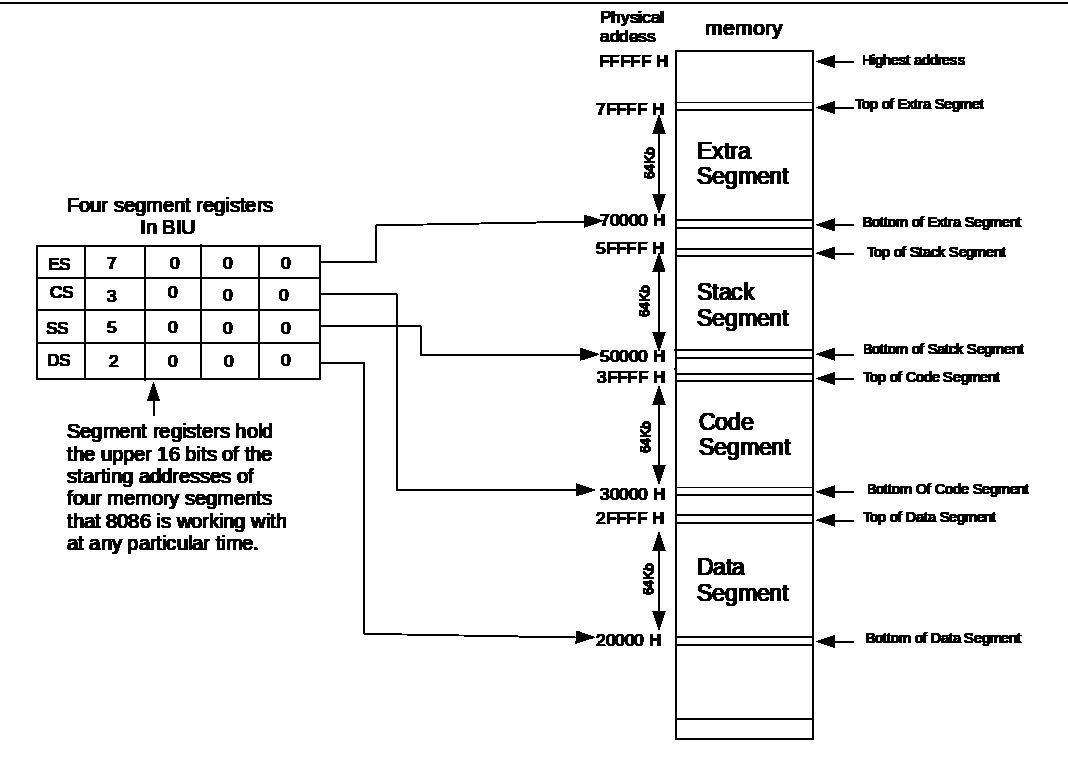
\includegraphics[height=10.5cm]{memory_segments.png}
	\caption{How segment registers map to memory locations.}
\end{figure}



\newpage
\subsection{Transition from real to protected mode}

When the system boots up and enters BIOS, it runs in \emphasis{real mode}. In real mode, the system only has access to 1 MB of memory therefore needs a 20-bit data bus (lines A0-19). Predecessors of the 8086 were only using 1 MB of RAM, so a 20-bit data address would suffice to run applications. When these applications were ported to newer architectures than can access more than 1 MB of RAM, the line A20 had to be turned off for compability reasons.

% prot mode ref https://www.byclb.com/TR/Tutorials/microprocessors/ch2_1.htm
Real mode prevents the registers from pointing to physical addresses larger than 1 MB. That means that whatever address is generated by $SEG*16+OFF$ is always truncated to its lower 20 bits ($2^{20}$ = 1 MB). Real mode therefore enables lines A0-19 and keeps A20 disabled, since the highest accessible address in real mode is $(2^{16}-1)\cdot 16+(2^{16}-1) = 2^{20} - 2^4 + 2^{16} - 1 < 2^{21} $, which fits in 21 bits. In \emphasis{protected mode}, A20, 21, \ldots, depending on the available memory are enabled. Other tasks are also permormed, such as disabling BIOS interrupts, enabling the Global Descriptor Table with segment descriptors suitable for code, data, and stack. More details about how protected mode starts in \TODO[ref]. Let's see an example.

% ref https://www.quora.com/What-is-the-A20-gate-in-a-CPU
For example, when \mintinline{latex}{0xFFFF:0x000F=0xFFFFF}, which fits in 20 bits. If the offset is increased by l, the address is \mintinline{latex}{0xFFFF:0x0010} which is \mintinline{latex}{0x100000} (more than 20 bits)! In this case, 8086 will wrap around the address by removing bit 20, so \mintinline{latex}{0xFFFF:0x0010} shall refer to byte \mintinline{latex}{0x00000}, \mintinline{latex}{0xFFFF:0x0011} shall refer to $0x00001$, and so on.


\newpage
\section{Location and role of reset vector}

% ref https://stackoverflow.com/a/32721444
After power up, all x86 CPUs are in real mode but with a strange behaviour until a CS assignment is found! As already mentioned, for the 80386 and later CPUs, the following data are defined in the registers during after power up:
\begin{minted}{latex}
IP          0xfff0
CS base     0xffff0000
CS selector 0xf000
\end{minted}
When fetching a new instruction (being in whatever mode: real, protected, etc) it seems that the hardware addressing logic is always using some CS cache register values to figure out what address to place on the Address Bus pins. The next instruction is:
\begin{minted}{latex}
Next_Instruction_Address_on_Bus= CS_segment_start_address + EIP
\end{minted}
Substututing the CS and EIP values, we get that the boot instruction is \mintinline{latex}{FFFF0000H + 0000FFF0H = FFFFFFF0H}. This is 16 bytes below 4 GM, so have we left real mode? This calculated address only contains  far jump to the memory location mapped to the system BIOS entry point (0x0000: 0x000F0000h).
The value where we jump, if \mintinline{latex}{CS=XYZW H}, is (use the left shift formula) \mintinline{latex}{000X YWZ0 + CSselector}, which is whithin the 1 MB area. For example, \mintinline{latex}{CS=0xf000, IP=0xe05b}, the the next ip (instruction pointer) is   \mintinline{latex}{0xfe05b = 0xf000*16 + 0xe05b} (real mode). The jump is illustrated below.
% ref example https://tc.gts3.org/cs3210/2016/spring/l/lec02.pdf

\begin{figure}[H]
	\centering
	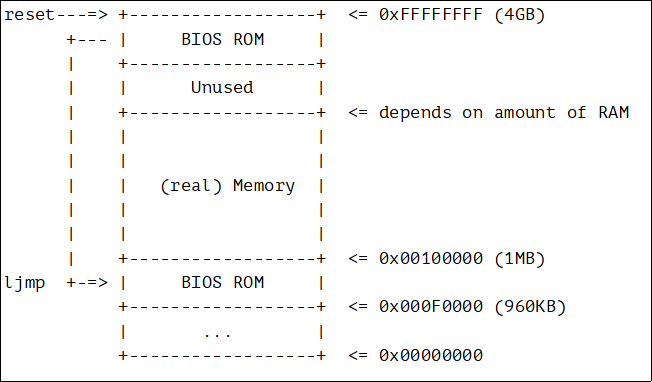
\includegraphics[height=5.5cm]{bios_jump.png}
	\caption{The jump from the ``reset vector'' (top of RAM) to BIOS entry point.}
\end{figure}
To summarise;
\begin{definition}
	The point in RAM pointed after power on which contains the instruction that jumps to the BIOS entry point is called \emphasis{reset vector}. 
\end{definition}

This behaviour is to assure that the power-up code will always be at the last corner of RAM. That way it will leave alone plenty of RAM for future OS disposal
% see also https://stackoverflow.com/questions/22312428/what-memory-is-used-for-storing-the-reset-vector


\newpage
\section{The MBR partition}

After jumping in the BIOS entry point, the BIOS starts. A lot of devices use MBR layout for the boot code.

% ref https://developer.ibm.com/tutorials/l-lpic1-102-1/, https://www.minitool.com/lib/boot-sector.html
Traditionally, a hard drive is formatted into 512 byte sectors (although larger sectors, such as 4 kB have recently been introduces). All the sectors on a disk platter that can be read without moving the head constitute a track. Disks usually have more than one platter. The collection of tracks on the various platters that can be read without moving the head is called a cylinder. The geometry of a hard drive is expressed in cylinders, tracks (or heads) per cylinder, and sectors/track.

\begin{definition}
	Cylinder 0, head 0 and sector 1 of hard disk are called master boot sector, which is also called \emphasis{master boot record} (MBR). This record takes up 512 bytes.
\end{definition}
When hard disk starts, it is used to transfer system control right to the certain operating system partition which is user-specified and registered in partition table. The content of MBR is written into the certain sector by partitioning software when it partitions. MBR doesn't belong to any operating system and doesn't change with the changes of operating systems. More details about the MBR booting process in the next section.


\subsection{How does the x86 MBR BIOS boot?}
% ref https://www.chromium.org/chromium-os/chromiumos-design-docs/disk-format?tmpl=%2Fsystem%2Fapp%2Ftemplates%2Fprint%2F&showPrintDialog=1
Legacy boot for x86 Linux has three steps:
\begin{enumerate}
\item The BIOS looks at the first block of each drive until it finds a Master Boot Record (MBR). This consists of 440 bytes of real-mode code, 6 ignored bytes, 4 instances of 16-byte primary partition records, and 2 signature bytes, 0x55 and 0xAA. That's 512 bytes. BIOS copies this block into RAM and starts executing the first byte. This all happens in x86 Real Mode.
\item Those first 440 bytes of MBR code are responsible for bootstrapping the rest of the OS. It searches the four partition table entries, finds a partition flagged as bootable, copies the first 512 bytes  from that partition (the so-called Volume Boot Record or VBR) into RAM, and jumps there. That code then continues the boot process in some unspecified way -- typically that VBR code (as well as the MBR code) is generated by and installed by grub, lilo, syslinux, or some similar bootloader.
\item The bootloader code identifies the kernel. It also creates a special table. The kernel eventually jumps to the its 32-bit entry point. This step is out of scope and won't be discussed further.
\end{enumerate}


\subsection{The structure of MBR}

 The ``master boot record'' has only 512 bytes and can't put too much. Its main function is to tell the computer where to find the operating system. It consists of three parts:

\begin{enumerate}
	\item 1-446 bytes: Call the machine code of the operating system.
	\item 447-510 bytes: Partition table (64 bytes).
	\item 511-512 bytes: Master boot record signature bytes (\mintinline{latex}{0x55} and \mintinline{latex}{0xAA}). 
\end{enumerate}

% ref http://glennastory.net/boot/mbr.html
The code (bytes 1-446) This code searches the Partition Table to find the first partition that is marked as an "active"or boot partition. Among them, the second part of the ``partition table'' is to divide the hard disk into several areas. 


\subsection{More about the partition table}

% ref http://www.ntfs.com/partition-table.htm
The partition table is a 64-byte data structure located in the same sector as the Master Boot Record (cylinder 0, head 0, sector 1). The Partition Table conforms to a standard layout that is independent of the operating system. Each Partition Table entry is 16 bytes long, making a maximum of four entries available. Each entry starts at a predetermined offset from the beginning of the sector, as follows:

\begin{itemize}
	\item Partition 1 -- starts at \mintinline{latex}{0x01BE (446)}
	\item Partition 2 -- starts at \mintinline{latex}{0x01CE (462)}
	\item Partition 3 -- starts at \mintinline{latex}{0x01DE (478)}
	\item Partition 4 -- starts at \mintinline{latex}{0x01EE (494)}
\end{itemize}
This is why MBR can only support up to four partitions. Recall that the last two bytes in the sector are its signature word and are always \mintinline{latex}{0x55 0xAA}.

% partition table example: http://thestarman.narod.ru/asm/mbr/STDMBR.htm
% TODO: see https://thestarman.pcministry.com/asm/mbr/PartTables.htm



\newpage
\section{Nasm assembly -- the \$ and \$\$ symbols}

The bootloader code used some Nasm 8086 assembly instructions whose usage may not be too obvious. This section explains how to use them.

\subsection{The structure of a Nasm program}

Memory segments (sections) need to be explicitely declared in a Nasm program. At least the text section is required.
\begin{figure}[H]
	\centering
	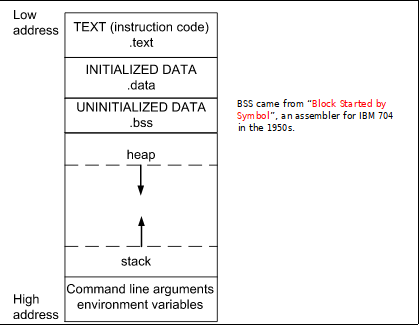
\includegraphics[height=6cm]{mem_segments.png}
	\caption{Memory segments diagram.}
	\label{fig:mem_segments}
\end{figure}

Data segment contains initialised data (variables), BSS segment contains unitialised data (reserved memory) and the text segment contains the code as well as the entry point for the linker, i.e. the label for the main program. This label is defined in the TEXT section and is \mintinline{latex}{_start} if \mintinline{latex}{ld} is used as linker or \mintinline{latex}{main} if \mintinline{latex}{gcc} is used as linker. The code below is borrowed from \cite{nasmtut}. In this case the former linker was preferred.

\lstinputlisting[language=nasm,style=nasm,caption={Nasm program skeleton - invokes exit interrupt. (\detokenize{src/empty.nasm)}.}, label=src:empty]{src/empty.nasm}


More examples found here \cite{nasmtut2}.


\subsection{The \$ notation}

\$ denotes the address of the current instruction, to be specific \$ evaluates to the assembly position at the beginning of the line containing the expression. 

\subsection{Uses of \$ -- string length}

\$ can be used measures the length of a string when defining the variables in the .data section. Simply subtract from it the address of the last defined variable.
\begin{minted}{nasm}
SECTION .data
msg     db 'Hello World!', 0Ah  
msg_len equ $ - msg
\end{minted}
equ is equivalent to the define macro in C, so it would just replace \mintinline{latex}{msg_len} with whatever is on the right hand side and db allocates space in memory. The complete ``Hello world'' program that uses the \$ notation is listed below.
\lstinputlisting[language=nasm,style=nasm,caption={Hello world in nasm using the \$ for string length. (\detokenize{src/hello.nasm)}.}, label=src:hello]{src/hello.nasm}
The latter code exists with segmentation error. To exit properly, the right interrupt needs to be used as listed here \cite{nasmtut} but we don't care about it in this case. 

\subsection{Uses of \$ -- jump to address}

\$ can also be used to instruct the EIP (Extended Instruction Pointer register, Extended meaning 32-bit) where to jump to relatively to the current instruction. As \$ stores the EIP (address of ``here''), doing \mintinline{latex}{jmp $+offset} jumps a number of lines lower in the code and  \mintinline{latex}{jmp $-offset} jumps a number of line higher in the code. Doing \mintinline{nasm}{jmp $} results in an infinite loop. To sum up, it's an alternative way of using the \mintinline{latex}{goto} instruction.

However, jumping by using \$ isn't very practical as to jump to a certain location we need to know how many bytes are used for each instruction. Jumping to a label is preferred. For example in Nasm, \mintinline{latex}{mov} instructions take 5 bytes and an \mintinline{latex}{int} takes 2 bytes. This is demonstrated in the code below, which runs an infinite loop that prints a string. \mintinline{latex}{jmp $-22} jumps one \mintinline{latex}{int} (interrupt) instruction and 4 \mintinline{latex}{mov} instructions up, to \mintinline{latex}{mov edx, msg_len}. We jump all the way up before all register assignments as \mintinline{latex}{int} overwrites them. 

\lstinputlisting[language=nasm,style=nasm,caption={Some code that performs jump using the \$ notation (\detokenize{src/jump.nasm)}.}, label=src:jump]{src/jump.nasm}


\subsection{The \$\$ symbol}

From \cite{nasmdoc}; \$\$ evaluates to the beginning of the current
section (.text, .data, etc.) and since \$ evaluates the (absolute) address of the ``here'', \mintinline{latex}{$ - $$} calculates how far we are in the current section.

\subsection{\mintinline{latex}{times} instruction}

Again, from \cite{nasmdoc}; the \mintinline{latex}{times} prefix causes the instruction to be assembled multiple times. For example, to fill 64 zeros in the memory: 
\begin{minted}{asm}
zerobuf:        times 64 db 0
\end{minted}
ut  \mintinline{latex}{times} is more versatile than that. The argument to \mintinline{latex}{times} is not just a numeric constant, but a numeric expression. It can evaluate mathematical operations including the address of ``here'' (\$). For example, to pad a string with the ``.'' character until it's 32 bytes long, the following can be done.

\begin{minted}{nasm}
msg     db     'in the loop!', 0Ah
        times 32-$+msg db '.'
msg_len equ    $-msg
\end{minted}

Note that because 8086 processor model is \emphasis{little endian}, the last defined bytes will be stored first. So the snippet above will \textit{prepend} ``.'' characters before the string.

The snippet below builds on \mintinline{latex}{jump.asm} and prints prepends dots until the string to be printed is 32 bytes (in this case 32 characters). It continuously prints \mintinline{latex}{...................in the loop!}.

\lstinputlisting[language=nasm,style=nasm,caption={A usage of the times instruction; pad a variable up to a length (\detokenize{src/times.nasm)}.}, label=src:times]{src/times.nasm}

Finally, \mintinline{latex}{times} can be used to repeat simple instructions by making trivial unrolled loops \cite{nasmdoc}, for instance:

\begin{minted}{asm}
times 100 movsb
\end{minted}


\subsection{Nasm compiling tips}

The following commands were used for the \mintinline{latex}{src/*.nasm} files to produce debuggable executable files.
\begin{minted}{bash}
nasm -f elf -g -F dwarf jump.nasm # compile
ld -m elf_i386 jump.o -o jump # link
gdb ./jump
./jump
\end{minted}



\newpage
\printbibliography


\end{document}
